\documentclass[11pt,letterpaper]{article}
\usepackage{graphicx, subcaption}
\usepackage[margin=1in]{geometry}
\usepackage{amsfonts,amsmath,amssymb,amsthm}
\usepackage{wasysym}
\usepackage{tikz}
\usepackage[english]{babel}
\usepackage[autostyle]{csquotes}

\newtheorem{thm}{Theorem}[section]
\newtheorem{lem}[thm]{Lemma}
\newtheorem{cor}[thm]{Corollary}
\newtheorem{prop}[thm]{Proposition}
\theoremstyle{definition}
\newtheorem{ex}[thm]{Example}
\newtheorem{rmk}[thm]{Remark}
\newtheorem{defn}[thm]{Definition}
\newtheorem{exer}[thm]{Exercise}

\newcommand{\N}{\mathbb{N}}
\newcommand{\Q}{\mathbb{Q}}
\newcommand{\R}{\mathbb{R}}
\newcommand{\Z}{\mathbb{Z}}

\begin{document}
\pagestyle{plain}

\vspace{.7cm}\begin{center}\vspace{-1cm}
\textbf{\large Results}\\

\end{center}

\hrule

%%%%%%%%%%%%%%%%%%

\begin{center}\section{Minimal Partition Size for $S=\langle m,m+1,...,2m-5\rangle$}\end{center}

\begin{defn}
    Let $S$ be a numerical semigroup. We use $\mathcal{P}(S)$ to denote the set of sizes of partitions with hook set $\mathbb{N} \setminus S$.
\end{defn}

\begin{lem}
    \label{Frob}
    Let $S$ be a numerical semigroup of the form $S=\langle m,m+1,m+2,...,2m-5\rangle$ with $m\geq 9$. Then the Frobenius number of $S$ is $F(S)=2m-1$.
\end{lem}

\begin{proof}
    We recall that the Apery set is the set of the minimal element of each residue class $\bmod$ $m$. Clearly, the smallest element in $S$ congruent to $0$ is $0$, and the smallest elements in $S$ congruent to $1, 2, ..., m-5$ are the minimal generators $m+1, m+2, ..., 2m-5$. We note that the smallest element of $S$ larger than $2m-5$ is $2m$, since $m$ is the smallest minimal generator. That is, $2m-4,2m-3,2m-2,2m-1$ are not elements of $S$. Since $m \geq 9$, $2m-5 \geq m + 4$. So $m+1, m+2, m+3, m+4$ are all generators of $S$. Adding the generator $2m-5$ to these, we obtain that $3m-4, 3m-3, 3m-2, 3m-1\in S$, which cover the remaining residue classes $\bmod$ $m$. Hence, 
    $$Ap(S,m)=\{0,m+1,...,2m-5,3m-4,3m-3,3m-2,3m-1\}.$$
    Finally, we note that $\max Ap(S, m) = 3m-1$, so $F(S) = (3m-1)-m = 2m-1$, as desired.
    
\end{proof}     

\begin{defn}[Frobenius triangle]
    Let $S$ be a numerical semigroup. A \textbf{Frobenius triangle} is a 3-tuple $(P, x,y)\in PF(S) \times \mathcal{M}(S) \times \mathcal{M}(S)$ such that $P+x+y =F(S)$. That is, $P+x = \overline{y}=F(S) -y$.

    An order ideal $I$ \textbf{satisfies the Frobenius triangle} $(P, x, y)$ if $P, x \in I$ and $\overline{y} \notin I$.
\end{defn}

\begin{lem}
    \label{Ideal}
    If $I$ is an order ideal of $S$ and for each $P\in I\cap PF(S)$, $P$ satisfies at least one of the following 
    \begin{enumerate}
        \item $2P\notin S$
        \item $F-P\in I$
        \item There is a Frobenius triangle $(P,x,y)$ satisfied by $I$
    \end{enumerate}
    Then we have that $A(S\cup I)\subseteq S$.
\end{lem}

\begin{prop}
    Let $S$ be a numerical semigroup of the form $S=\langle m,m+1,m+2,...,2m-5\rangle$ where $m\geq 9$. Then

    $$\lim_{m\to\infty}\frac{\min \mathcal{P}(S)}{|\lambda(S)|} = \frac{4}{5}$$

    where $\lambda(S)$ is the enumeration of $S$. 

\end{prop}

\begin{proof}
    Using Lemma \ref{Frob} above we can conclude that the set of gaps for $S$ is 
    \[\mathcal{H}=\{1,2,...,m-1,2m-4,2m-3,2m-2,2m-1\}\]
    From this it is simple to see that the void of $S$ is 
    \[\mathcal{M}=\{1,2,3,2m-4,2m-3,2m-2\}\]
    Constructing the void poset gives us 
    \begin{center}
    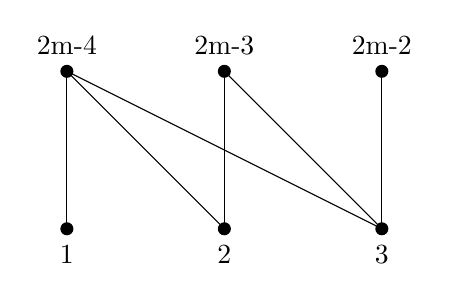
\begin{tikzpicture}

    \coordinate (A) at (0,0);
    \coordinate (B) at (2,0);
    \coordinate (C) at (4,0);
    \coordinate (D) at (0,2);
    \coordinate (E) at (2,2);
    \coordinate (F) at (4,2);

    \draw (A) -- (D);
    \draw (D) -- (B);
    \draw (D) -- (C);
    \draw (E) -- (B);
    \draw (E) -- (C);
    \draw (F) -- (C);

    \node at (A) [circle, fill, scale=0.5, label=below:{1}] {};
    \node at (B) [circle, fill, scale=0.5, label=below:{2}] {};
    \node at (C) [circle, fill, scale=0.5, label=below:{3}] {};
    \node at (D) [circle, fill, scale=0.5, label=above:{2m-4}] {};
    \node at (E) [circle, fill, scale=0.5, label=above:{2m-3}] {};
    \node at (F) [circle, fill, scale=0.5, label=above:{2m-2}] {};
    
        
    \end{tikzpicture}
    \end{center}

    Using the void poset we note that the only order ideals that satisfy Lemma \ref{Ideal} are 
    \[\emptyset,\quad \mathcal{M}, \quad \{1,2m-4,2m-2\},\quad \{2,2m-4,2m-3\},\quad \{1,2m-4\},\quad \{1,2,2m-4,2m-3\}\]
    This is due to $2m-3$ and $2m-2$ not satisfying either condition 1 or 3 thus including either of these elements forces the order ideal, $I$, to contain 2 or 1 respectively. Additionally if $P=2m-4$ and $I$ contains at least one of 1 or 2 and does not contain at least one of $2m-3$ or $2m-2$ (which one to not include is dependent on the choice of 1 or 2 to include in $I$) then $I$ does satisfy a Frobenius triangle.

    We can now construct the Ferr diagrams of $S$ and $S\cup I$ for each order ideal above.

    \begin{center}
        \begin{tikzpicture}
        
            \coordinate (A) at (0,0);
            \coordinate (B) at (0,2);
            \coordinate (C) at (0,3.5);
            \coordinate (D) at (.5,0);
            \coordinate (E) at (.5,2);
            \coordinate (F) at (3,2);
            \coordinate (G) at (3,3.5);
            \coordinate (H) at (0.23,1);

            \draw (A) -- (C);
            \draw (A) -- (B);
            \draw (A) -- (D) node[midway, below] {0};
            \draw (D) -- (E);
            \draw (B) -- (E);
            \draw (B) -- (F);
            \draw (F) -- (G);
            \draw (G) -- (C) node[midway, above] {$S$};

            \node at (1.5,2.75) {$4m-12$};
            \node at (0.7,1.8) {$m$};
            \node at (2.7,1.8) {$2m-5$};
            \node at (H) {\rotatebox{90}{$m-1$}};

            \coordinate (I) at (5,2);
            \coordinate (J) at (7,2);

            \draw [>=latex, <->, line width=2pt, scale=2] (I) -- (J);

            \coordinate (K) at (12.5,3);
            \coordinate (L) at (10.5,3);
            \coordinate (M) at (9,3);
            \coordinate (N) at (12.5,2.5);
            \coordinate (O) at (10.5,2.5);
            \coordinate (P) at (10.5,0);
            \coordinate (Q) at (9,0);
            \coordinate (R) at (11.5,2.77);

            \draw (K) -- (M) node[midway, above] {$S\cup \mathcal{M}$};
            \draw (K) -- (L);
            \draw (K) -- (N);
            \draw (N) -- (O) node[midway, above] {$m-1$};
            \draw (L) -- (O);
            \draw (L) -- (P);
            \draw (P) -- (Q);
            \draw (Q) -- (M);

            \node at (9.75,1.5) {$4m-12$};
            \node at (9.2,-0.25) {0};
            \node at (10.7,0.25) {4};
            \node at (10.8, 2.3) {$m$};
            \node at (12.5,2.3) {$2m-2$};
            \node at (13.2,2.75) {$2m-1$};

            
        \end{tikzpicture}
    \end{center}

    Notice that these are transposition of each other thus the sizes are the same giving us that \[|\lambda(S)|=|\lambda(S\cup\mathcal{M})|=5m-13\]

    \begin{center}
        \begin{tikzpicture}
        
            \coordinate (A) at (0,0);
            \coordinate (B) at (0,2);
            \coordinate (C) at (0,3.5);
            \coordinate (D) at (.8,0);
            \coordinate (E) at (.8,2);
            \coordinate (F) at (3,2);
            \coordinate (G) at (3,3.5);
            \coordinate (H) at (0.4,1);
            \coordinate (1) at (3,2.75);
            \coordinate (2) at (3.7,2.75);
            \coordinate (3) at (3.7,3.5);

            \draw (A) -- (C);
            \draw (A) -- (B);
            \draw (A) -- (D);
            \draw (D) -- (E);
            \draw (B) -- (E);
            \draw (B) -- (F);
            \draw (F) -- (G);
            \draw (G) -- (C) node[midway, above] {$S\cup \{1,2m-4,2m-2\}$};
            \draw (1) -- (2) -- (3) -- (C);

            \node at (1.5,2.75) {$2m-2$};
            \node at (1,1.8) {$m$};
            \node at (2.7,1.8) {$2m-4$};
            \node at (H) {\rotatebox{90}{$2m-4$}};
            \node at (.2,-.2) {0};
            \node at (1,.2) {2};

            \coordinate (I) at (5,2);
            \coordinate (J) at (7,2);

            \draw [>=latex, <->, line width=2pt, scale=2] (I) -- (J);

            \coordinate (K) at (12.5,3);
            \coordinate (L) at (10.5,3);
            \coordinate (M) at (9,3);
            \coordinate (N) at (12.5,1.9);
            \coordinate (O) at (10.5,1.9);
            \coordinate (P) at (10.5,0);
            \coordinate (Q) at (9,0);
            \coordinate (R) at (11.5,2.77);
            \coordinate (11) at (9,-.8);
            \coordinate (22) at (9.75,-.8);
            \coordinate (33) at (9.75,0);
            

            \draw (K) -- (M) node[midway, above] {$S\cup \{2,2m-4,2m-3\}$};
            \draw (K) -- (L);
            \draw (K) -- (N);
            \draw (N) -- (O);
            \draw (L) -- (O);
            \draw (L) -- (P);
            \draw (P) -- (Q);
            \draw (Q) -- (M);
            \draw (11) -- (Q);
            \draw (11) -- (22) -- (33);


            \node at (9.75,1.5) {$2m-2$};
            \node at (9.35,-1) {0};
            \node at (10.15,-.25) {2};
            \node at (10.7,0.25) {3};
            \node at (10.75, 1.7) {$m$};
            \node at (12.5,1.7) {$2m-3$};
            \node at (13.2,2.75) {$2m-1$};
            \node at (11.5,2.45) {$2m-4$};

            
        \end{tikzpicture}
    \end{center}

    Again note that these are transposition of each other thus the sizes are the same giving us that \[|\lambda(S\cup \{1,2m-4,2m-2\})|=|\lambda(S\cup\{2,2m-4,2m-3\})|=4m-5\]

    \begin{center}
        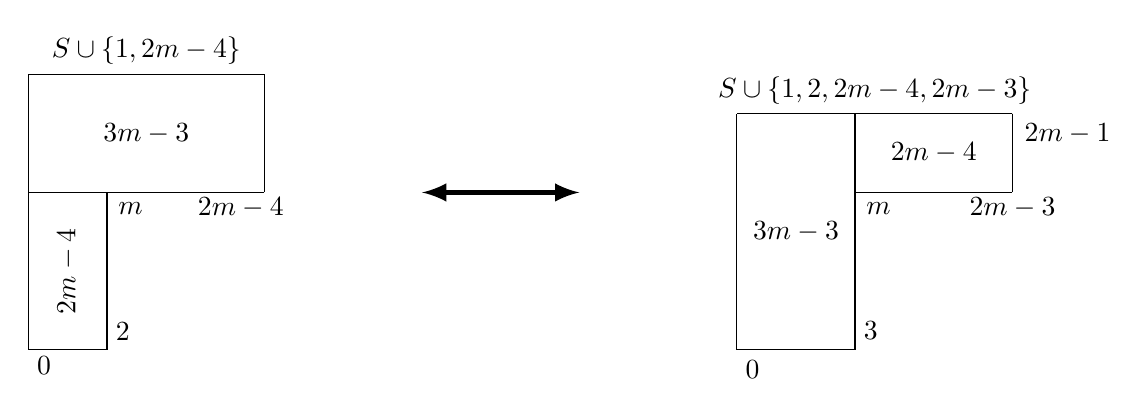
\begin{tikzpicture}
        
            \coordinate (A) at (0,0);
            \coordinate (B) at (0,2);
            \coordinate (C) at (0,3.5);
            \coordinate (D) at (1,0);
            \coordinate (E) at (1,2);
            \coordinate (F) at (3,2);
            \coordinate (G) at (3,3.5);
            \coordinate (H) at (0.23,1);

            \draw (A) -- (C);
            \draw (A) -- (B);
            \draw (A) -- (D);
            \draw (D) -- (E);
            \draw (B) -- (E);
            \draw (B) -- (F);
            \draw (F) -- (G);
            \draw (G) -- (C) node[midway, above] {$S\cup\{1,2m-4\}$};

            \node at (1.5,2.75) {$3m-3$};
            \node at (1.3,1.8) {$m$};
            \node at (2.7,1.8) {$2m-4$};
            \node at (.5,1) {\rotatebox{90}{$2m-4$}};
            \node at (.2,-.2) {0};
            \node at (1.2,.23) {2};

            \coordinate (I) at (5,2);
            \coordinate (J) at (7,2);

            \draw [>=latex, <->, line width=2pt, scale=2] (I) -- (J);

            \coordinate (K) at (12.5,3);
            \coordinate (L) at (10.5,3);
            \coordinate (M) at (9,3);
            \coordinate (N) at (12.5,2);
            \coordinate (O) at (10.5,2);
            \coordinate (P) at (10.5,0);
            \coordinate (Q) at (9,0);
            \coordinate (R) at (11.5,2.77);

            \draw (K) -- (M) node[midway, above] {$S\cup\{1,2,2m-4,2m-3\}$};
            \draw (K) -- (L);
            \draw (K) -- (N);
            \draw (N) -- (O);
            \draw (L) -- (O);
            \draw (L) -- (P);
            \draw (P) -- (Q);
            \draw (Q) -- (M);

            \node at (9.75,1.5) {$3m-3$};
            \node at (9.2,-0.25) {0};
            \node at (10.7,0.25) {3};
            \node at (10.8, 1.8) {$m$};
            \node at (12.5,1.8) {$2m-3$};
            \node at (13.2,2.75) {$2m-1$};
            \node at (11.5,2.5) {$2m-4$};

            
        \end{tikzpicture}
    \end{center}

    Finally the sizes of these are 
    \[|\lambda(S\cup \{1,2m-4\})|=|\lambda(S\cup\{1,2,2m-4,2m-3\})|=5m-7\]

    Now it is trivial to see that $\{1,2m-4,2m-2\}$ is an order ideal that gives us our minimum partition size of $4m-5$ and $S$ has partition size of $5m-13$ giving us our final result of 
    \[\lim_{m\to\infty}\frac{\min \mathcal{P}(S)}{|\lambda(S)|} = \lim_{m\to\infty}\frac{4m-5}{5m-13} =\frac{4}{5}\]
    
\end{proof}

\newpage

%%%%%%%%%%%%%%%%%%%%%%%%%
\begin{center}
    \section{Minimal Partition Size for $S=\{0,k,...,nk\rightarrow\}$}
\end{center}

\begin{lem}
    \label{n=1 case}
    Let $k\in\Z^+$. For all numerical semigroups of the form $S=\{0,k\rightarrow\}$ we have that $\min\mathcal{P}(S)=|\lambda(S)|=k-1$.
\end{lem}

\begin{proof}
    Each partition that correlates to a value in $\mathcal{P}(S)$ must have the hook set $\{1,2,...,k-1\}$. Thus there must be at least $k-1$ boxes in the Young diagram. Since $|\lambda (S)|=k-1$ we have that $\min\mathcal{P}(S)=|\lambda(S)|$.
\end{proof}




%\begin{lem}
    %\label{line poset}
    %For numerical semigroups of the form $S=\{0,k,...,kn\rightarrow\}$ the void poset diagram is made of disjoint lines each with $n$ height and each point in a line is equivalent modulo $k$.
%\end{lem}


\begin{lem}
    \label{line poset lem}
    For all self dual order ideals $I$ of $S=\{0,k,...,nk\rightarrow\}$ if $x\in I$ then $I$ contains all elements less then $F(S)$ equivalent to $x$ modulo $k$.
\end{lem}

\begin{proof}
     First see $x\in\mathcal{M}$ if and only if $x\notin S$ and $F-x\notin S$. Note that $1,2,...,k-1$ are all not in $S$ and that for $x\in\{0,1,...,k-1\}$, $F(S)-x=nk-1\in S$ if and only if $nk-1-x=mk$ for some $m\in\Z^+$ thus $x\equiv k-1\mod k$. Giving us that all elements smaller than $F(S)$ that are congruent to $1,2,...,k-2$ modulo $k$ are in the void of $S$. Now notice that $x\preccurlyeq y$ if and only if $y-x\in S$ and all elements in $S$ are equivalent to 0 modulo $k$ thus $x\equiv y\mod k$. Therefore the void poset will be made of $k-2$ lines of height $n$ where each line contains elements of one congruence class. Since $I$ is an order ideal if $x\in I$ then $I$ must contain the largest element congruent to $x$ in the void of $S$, call this $X$. Since $I$ is self dual then it also contains $F(S)-X\equiv 6-X\mod k$ and as before also contains all elements larger than and congruent to $F(S)-X$ of which live in the void, call this $Y$. But then since $I$ is self dual again we must have that $F(S)-Y\in I$ and note that $F(S)-Y\equiv 6-6-X\equiv X\mod k$ but also $0<F(S)-Y<k$ since $(n-1)k<Y<nk$ thus we must also have all smaller elements then $x$ that are congruent to $x$ modulo $k$. Giving us that any self dual order ideal will have all elements less than $F(S)$ and congruent to $X$ and $Y$ modulo $k$.
\end{proof}




\begin{prop}
    Let $n,k\in\Z^+$. For all numerical semigroups of the form $S=\{0,k,2k,...,nk\rightarrow\}$ if $I$ a self dual order ideal such that $A(S\cup I)=A$ then $|\lambda(S\cup I)|\geq |\lambda(S)|$. 
\end{prop}

\begin{proof}
    Given an order ideal $I$ of $S$ such that $A(S\cup I)=S$ break up the Young diagram of $S\cup I$ as follows. Find the first box above each of $0,k,2k,...,nk$ then draw a vertical and horizontal lines that goes through the bottom left corner of each box. It is not difficult to see that there are $k$ vertical "floors" of this diagram. From Lemma \ref{line poset lem} we note that the right most section of each floor are the same since our right steps in the Young diagram occur at the same time due to our ideal containing all elements in a specific equivalence class of $k$. From Lemma \ref{n=1 case} these sections have size at least $k-1$. By construction all other sections should be rectangles with the same base, $b$, and height, $h$. Additionally, since the base is the number of non gaps from the previous floor and the height is the number of gaps from the current floor and the profile of each floor covers all the residue classes modulo $k$ we have that $b+h=k$. This then implies that $b\cdot h\geq k-1$. If we break up the Young diagram of $\lambda(S)$ the same way we note that we have $\frac{n(n+1)}{2}$ rectangles of size $k-1$. Since we have shown that all sections of $\lambda(S\cup I)$ have size at least $k-1$ then clearly we have $|\lambda(S\cup I)|\geq |\lambda(S)|$.
\end{proof}




%\begin{lem}
   % \label{modulo k}
   % For all self dual order ideals $I$ of $S=\{0,k,...,nk,nk+s+1\rightarrow\}$ if $x\in I$ then $I$ contains all element less than $nk$ congruent to $x$ modulo $k$.
%\end{lem}

%\begin{proof}
    
%\end{proof}





%\begin{cor}
 %   \label{top row}
   % For all self dual order ideals $I$ of $S=\{0,k,...,nk,nk+s+1\rightarrow\}$ if $x\in I$ and $x\in (nk,nk+s+1)$ then $I$ contains all element less than $nk$ congruent to $x$ modulo $k$.
%\end{cor}

%\begin{proof}
    
%\end{proof}





%\begin{lem}
  %  \label{area}
%    If $r,s\geq 2$ and $r+s=k$ then $r\cdot s\geq 2k-4$.
%\end{lem}

%\begin{proof}
    
%\end{proof}





%\begin{lem}
  %  \label{height 2}
  %  Given a self dual order ideal $I$ of $S=\{0,k,...,nk,nk+s+1\rightarrow\}$ $I$ will not cover at least 2 residue classes modulo $k$.
%\end{lem}

%\begin{proof}
    
%\end{proof}




%\begin{prop}
  %  Let $n,k,s\in \Z^+$ where $0\leq r\leq k-2$. For all numerical semigroups of the form $S=\{0,k,2k,...,nk,nk+s+1\rightarrow\}$ if $I$ is a self dual order idea such that $A(S\cup I)=A$ then we have that $|\lambda(S\cup I)|\geq|\lambda(S)|$.
%\end{prop}

%\begin{proof}
    %We will compare sections of $|\lambda(S\cup I)|$ and $|\lambda(S)|$ by breaking the Young diagram of each partition into sections. For all steps in the walk of each Young diagram that are equivalent to 0 modulo $k$ find the box above this step and draw a vertical and horizontal line starting from the bottom left corner and going through the entire diagram. For notational purposes number the rows $1,...,n+1$ starting from the bottom. 

   % To compare the area of the first $n$ rows we will consider two cases. For both cases let $I$ be a self dual order ideal and note that the first $n$ rows of $|\lambda(S\cup I)|$ will have the same right most section since Lemma \ref{modulo k} ensures the walks along these sections are the same.

   % \textbf{Case 1:} First we consider the area of $\lambda(S\cup I)$. If $I$ does not contain any $x$ such that $x\equiv -1\mod{k}$ then for the first $n$ consider the right most section. Since $I$ does not contain an element congruent to $-1$ modulo $k$ then the shape created by the walk along this section will have width $w$ and height $h$ such that $w+h=k$. Thus it follows that the area of these sections are at least $k-1$. Now we consider the rest of the rectangles in the first $n$ rows. Since $I$ is self dual the right most sections of the first $n$ rows are the same and thus given any section it must have the same width as some right most section of a row below it. Additionally it will have the same height as the right most section in the same row as itself. However these heights and widths are uniform for the first $n$ rows so we have that all sections below the top row have area at least $k-1$. For similar reasoning we can see that each section below the top row of $\lambda(S)$ will have area exactly $k-1$. 

    %\textbf{Case 2:} Now consider when $I$ does contain an $x$ such that $x\equiv -1\mod{k}$. The right most section of each of the first rows will be a shape with width $w$ and height $h$ such that $w+h=k-1$ since we cover all the residue classes of $k$ along the walk but the last step is cut off by the next row above it. Thus the area of these sections are at least $k-2$. for the rest of the blocks below the top row due to similar reasoning as in the previous case we note that the width of each block $w$ and height $h$ are such that $w+h=k$ but we also have that $w,h\geq 2$ since $I$ must contain at least one element giving us at least two right steps and it must not cover at least two congruency classes due to Lemma \ref{height 2} so we have at least two up steps. Therefore due to Lemma \ref{area} we see that they must have area at least $2k-4$. Starting with the first row take the right most section of row $a$ and $a+1$, and the block above the right most section of row $a$. The area of these three sections is $2(k-2)+(2k-4)=4k-8$. For the same sections in $\lambda(S)$ we get area $3(k-1)=3k-3$ which gives us that $4k-8\geq3k-3$ whenever $k\geq 5$ and $n\geq 2$. If $n$ is even we have enough rows to cover each other. If $n$ is odd we have row $n$ that cannot be covered by the row above it. For this row note that there are at least 3 sections. in $\lambda(S)$ the area is $3(k-1)=3k-3$. In $\lambda(S\cup I)$ the two block have area at least $2(2k-4)$ and the right most section has area at least $k-2$. Since $3k-3\leq 5k-10$ whenever $k\geq 5$ this second to last row in $\lambda(S\cup I)$ is at least as large as the one in $\lambda(S)$.
    
  %  Combining these cases we see that the area below the top row of $\lambda(S\cup I)$ is at least as large as the area below the top row of $\lambda(S)$.

  %  Now to deal with the top row. For $\lambda(S)$ we have width $n+1$ since we make exactly $n+1$ right steps in the walk and we have height $s$ since there are exactly $s$ gaps between $nk$ and $nk+s+1$. Thus the area is $(n+1)s$. For $\lambda(S\cup I)$ the right most section the walk will have $r+1$ steps thus the area is at least $r$. For the other blocks in the top row the width will be the width of the right most section of the row that lies below it. However this width is at least as large as the width of the right most section of the top row due to Corollary \ref{top row} and will have the same height as the right most section of the top row thus it will have area at least $r$ and since there are exactly $n+1$ sections the top row will have area at least $(n+1)r$ which is the same as $\lambda(S)$. Thus giving us our desired result. 
%\end{proof}


%%%%%%%%%%%%%%%%%%%%%
\newpage

\begin{center}
    \section{Ideals of $S=\{0,k,...,nk\rightarrow\}$}
\end{center}






\begin{lem}
    \label{poset nk}
    For the family of semigroups $S=\{0,k,...,nk\}$ the void poset is made of $k-2$ disjoint chains of height $n$ of which all elements lie in the same congruency classes of $k$ ranging from $1,2,...,k-2$.
\end{lem}

\begin{proof}
    
\end{proof}

\begin{defn}
    We call each of these chains a \textbf{void strand} for their respective congruency class modulo $k$.
\end{defn}





\begin{prop}
    For the family of semigroups $S=\{0,k,2k,...,nk\rightarrow\}$ we have that 
    \[\min\mathcal{P}(S)=|\lambda(S)|\]
\end{prop}

\begin{proof}
    Given an order ideal $I$ of $S$ that preserves hook lengths consider the young diagram of $\lambda(S\cup I)$ and $\lambda(S)$. Break up each diagram by drawing a horizontal and vertical line starting at the bottom left corner of the first box above each step in the walk congruent to $0$ modulo $k$. For $\lambda(S)$ it is not hard to see that by computing the hook lengths of each section modulo $k$ each section should get exactly one hook length for the residue classes $1,2,...,k-1$. We claim that in each section of $\lambda(S\cup I)$ there will be at least one hook length congruent to $1,2,...,k-1$ modulo $k$ thus each section of $\lambda(S\cup I)$ is at least as large as the corresponding section in $\lambda(S)$. First note that $F=kn-1\equiv -1\mod k$ and for notational sake call the portion of the walk below a specific section the bottom walk and the portion of the walk to the right of a section the right walk. For hook congruent to $k-1$ by definition the bottom walk of any section will contain an element congruent to $0$ modulo $k$ and the right section will have a gap congruent to $k-1$ modulo $k$ thus we can always ensure a hook congruent to $k-1$ exists. For a hook of $-2$ if the right walk has a gap at the element congruent to $k-2$ then we are done since the bottom walk will contain a step congruent to $0$. Assume that the right walk contains $a\equiv k-2\mod k$ thus $a\in I$. Then by the structure of the order ideal $I$ must contain the pseudofrobenius that covers $a$, call this $P$. Since $P=nk-2$ it cannot satisfy a Frobenius triangle, thus $I$ must contain $1$ and thus all the elements congruent to $1$ modulo $k$. Then we can take the gap congruent to $-1$ in the right walk and the element congruent to $1$ in the bottom walk to get a hook of $-2$. Therefore we can always obtain a hook of $-2$. For a hook of $-3$ again if the right walk has a gap congruent to $-3$ then we are done. So assume that the right walk contains a $b\equiv k-3 \mod k$ thus $b\in I$. Similarly $I$ must now contain the pseudofrobenius number $Q$ that covers $b$. Therefore either $2\in I$ -- in which case taking the gap congruent to $-1$ in the right step and the element in the bottom step congruent to $2$ will give us a hook congruent to $-3$ -- or $Q$ satisfies the Frobenius triangle $(Q,1,1)$ which implies that $1\in I$ and $F-1\notin I$. Which then gives us that $I$ contains all elements congruent to $1$ modulo $k$ and no elements congruent to $F-1\equiv -2 \mod k$. Thus taking the gap in the right walk congruent to $-2$ and the element in the bottom walk congruent to $1$ gives us a gap of $-3$. For a general hook length let $c$ be some congruency class $\{1,2,...,k-1\}$ if the right walk does not cover this congruency class we are done so assume that $c\in I$. Then $I$ must contain the pseudofrobenius number $PF$ that covers $c$. Since $I$ preserves hook lengths either $I\ni F-PF\equiv -1-c\mod k$ -- in which case $I$ contains all elements congruent to $-1-c$ modulo $k$ thus taking the gap in the right walk congruent to $-1$ and this element in the bottom walk gives a hook congruent to $-1-(-1-c)\equiv c\mod k$ -- or $PF$ satisfies a Frobenius triangle $(PF,x,y)$ where $x\in I$, $F-y\notin I$, and $PF+x+y=F$. Since $F-y$ is not in $I$ then $I$ contains no elements congruent to and since $x\in I$ then $I$ contains all elements larger then $x$ and congruent to $x$ modulo $k$. Therefore taking the gap in the right walk congruent to $F-y$ and the element in the bottom walk congruent to $x$ gives a hook length congruent to $(F-y)-x=PF\equiv c\mod k$. Thus giving us a hook length of the congruency classes $\{1,2,.,,,k-1\}$ in each section and finishing our proof.
\end{proof}



%%%%%%%%%%%%%%%%%%%%%
\newpage

\begin{center}
    \section{Ideals of $S=\{0,k,...,nk,nk+s+1\rightarrow\}$}
\end{center}




\begin{prop}
    For the family of semigroups $S=\{0,k,2k,...,nk,nk+s+1\rightarrow\}$ we have that 
    \[\min\mathcal{P}(S)=|\lambda(S)|\]
\end{prop}

\begin{proof}
    This is very similar to the proof above with some variation, namely drawing horizontal lines above $F-m$ but it almost follows directly.
\end{proof}



%%%%%%%%%%%%%%%%%%%%%
\newpage

\begin{center}
    \section{Self Dual Ideals}
\end{center}

\begin{prop}
    If $I$ is a self dual order ideal of $S$ then $|\lambda(S)|\leq|\lambda(S\cup I)|$
\end{prop}

\begin{proof}
    Recall that for a numerical semigroup $S$ if $T$ is a numerical set associated to $S$ where $T=S\cup I$ then \[|\lambda(T)|=|\lambda(S)|+|A|-|B|\] where the sets $A,B$ are defined as 
    \[A=\{(i,g):i\in I,g\notin T, i<g\}\quad\text{and}\quad B\{(s,i):s\in S,i\in I,s<i\}\]
    Now given that $I$ is a self dual order ideal of $S$ consider the function 
    \[f:B\rightarrow A, \quad (s,i)\mapsto (F-i,F-s)\]
    Since $I$ is self dual and $i\in I$ then $F-i\in I$. Note that $F-s\notin S$ otherwise $F-s=s'\implies F\in S$ which is a contradiction, also note that if $F-s\in I$ then $F-(F-s)=s\in I$ which is another contradiction thus $F-s\notin T$. Finally see that since $s<i$ then $F-i<F-s$ therefore our function $f$ is well defined. Trivially $f$ is injective thus we get our result that $|\lambda(T)|\geq |\lambda(S)|$.
\end{proof}



%%%%%%%%%%%%%%%%%%%%%
\newpage

\begin{center}
    \section{Type 3 stuff}
\end{center}




\begin{prop}
    If $S$ is a numerical semigroup of type 3 then for any numerical set $T$ associated to $S$ we have that $|\lambda(T)|\geq |\lambda(S)|$.
\end{prop}

\begin{proof}
    Let $S$ be a numerical semigroup of type 3. Suppose that $PF(S)=\{P,Q,F\}$ where $P<Q<F$. Then due to Theorem 6.5 in \textbf{Deepesh Paper} we have 4 cases.

    \textbf{Case 1:} If $P+Q-F\notin S$, then $P(S)=4$ where each $I$ is self dual. As we have shown for all self dual order ideals $|\lambda(S\cup I)|\geq |\lambda(S)|$ thus we are done.

    \textbf{Case 2:} If $P+Q-F\in S$ and $Q-P\notin\mathcal{M}(S)$, then $P(S)=2$. Since for all numerical semigroups there are always two ideals that produce numerical sets associated to $S$ namely the ideals $I=\emptyset,\mathcal{M}(S)$ then in this case these are the only two and they must have the same size since they are transposes of each other. Thus we are done.

    \textbf{Case 3:} If $P+Q-F$, $Q-P\in\mathcal{M}(S)$, and $F+P=2Q$, then $P(S)=3$. In this case the ideals are exactly 
    \[I=\emptyset, \mathcal{M}(S), \{x\in\mathcal{M}(S):Q-P\preccurlyeq x\}\]
    As above we can disregard the empty ideal and the ideal containing the whole void. For the following order ideal $I$ consider the sets $A,B$ and function $f$ defined below
    \[I=\{x\in\mathcal{M}(S):Q-P\preccurlyeq x\}\]
    \[A=\{(i,g):i\in I,g\notin T, i<g\} \quad\text{and}\quad B=\{(s,i):s\in S,i\in I,s<i\}\]
    \[f:B\rightarrow A, \quad (s,i)\mapsto (Q-i,Q-s)\]
    First we show that $Q-i$ is in the void. Assume that $Q-i\in S$, since $Q,i\in\mathcal{M}(S)$ this gives us that $i\preccurlyeq Q$. However since $Q-P\preccurlyeq i$ this implies that $Q-P\preccurlyeq Q\implies P\in S$ which is a contradiction thus \[Q-i\notin S\] Now assume that $F-(Q-i)\in S$ this gives us that $F-Q+i=\overline{Q}+i=Q-P+i\in S$. Since the maximum elements of the void poset are $Q$ and $P$ then $i$ must be covered by one of them. Since $\overline{Q}\preccurlyeq i$ we cannot have that $i\preccurlyeq Q$ otherwise $\overline{Q}\preccurlyeq Q\implies P\in S$. Thus $i\preccurlyeq P\implies P-i\in S$. Now since both $P-i$ and $Q-P+i$ are both in $S$ their sum $(P-i)+(Q-P+i)=Q\in S$ which is a contradiction thus 
    \[F-(Q-I)\notin S\]
    So from the previous two results we see that 
    \[Q-i\in\mathcal{M}(S)\]
    
    Now we show that $Q-i\in I$. Note that $Q-P\preccurlyeq Q-i \iff i\preccurlyeq P$. Assume that $i\not\preccurlyeq P$ then since $i$ must be covered by either $P$ or $Q$ we have that $i\preccurlyeq Q$ but we know that $Q-P\preccurlyeq i$ giving us that $Q-P\preccurlyeq Q$ again a contradiction. Thus $i\preccurlyeq P$ giving us that \[Q-i\in I\]
    
    Now we show that $Q-s$ in not in $T=S\cup I$. Clearly $Q-s\notin S$ since otherwise $Q\in S$, a contradiction. If $Q-s\in I$ then $Q-P\preccurlyeq Q-s\implies (Q-s)-(Q-P)=P-s\in S\implies P\in S$. Therefore \[Q-s\notin T\]
    So our function $f$ is well defined and is trivially injective thus we see that $|B|\leq |A|$. Recall that for a numerical semigroup $S$ if $T$ is a numerical set associated to $S$ where $T=S\cup I$ then $|\lambda(T)|=|\lambda(S)|+|A|-|B|$. Giving us for this case that $|\lambda(S)|\leq |\lambda(T)|$.

    \textbf{Case 4:} If $P+Q-F\in S$, $Q-P\in\mathcal{M}(S)$, and $F+P\neq 2Q$, then $P(S)=4$. With the ideals 
    \[I=\emptyset,\mathcal{M}(S),\{x\in\mathcal{M}(S):\overline{Q}\preccurlyeq x\},\{x\in\mathcal{M}(S):Q-P\preccurlyeq x\}\]
    Just as above we can disregard the empty ideal and the ideal containing the whole void since they will have the same size as $S$. For the ideal containing everything that covers $Q-P$ we can use the same function in part 3. Thus it suffices to show the result holds for the ideal 
    \[I_2=\{x\in\mathcal{M}(S):\overline{Q}\preccurlyeq x\}\]
    If we can show that the dual of $I_1=\{x\in\mathcal{M}(S):Q-P\preccurlyeq x\}$, namely the set
    $I^*_1=\{x\in\mathcal{M}(S):x\not\preccurlyeq\overline{Q-P}\}$ is equivalent to $I_2$ then we are done since the partitions of the numerical sets $S\cup I_1$ and $S\cup I_1^*$ have the same size and we know from case 3 that $|\lambda(S\cup I_1)|\geq |\lambda(S)|$. 

    First assume that $x\in I_2$ thus $\overline{Q}\preccurlyeq x$. For contradiction assume that $x\notin I_1^*$ thus $x\preccurlyeq\overline{Q-P}$. This gives us that $\overline{Q}\preccurlyeq\overline{Q-P}$ which implies that $F-(Q-P)-(F-Q)=P\in S$, a contradiction. So we have that 
    \[I_2\subseteq I_1^*\]
    Now using Lemma 6.3 from \textbf{Deepesh Paper} we have that if $x\not\preccurlyeq Q$ then $Q-P\preccurlyeq x$ which the contrapositive gives us that if $Q-P\not\preccurlyeq x$ then $x\preccurlyeq Q$. Taking the conjugates presents that $\overline{x}\not\preccurlyeq\overline{Q-P}$ implies that $\overline{Q}\preccurlyeq\overline{x}$ which is exactly saying that 
    \[I_1^*\subseteq I_2\]
    We have shown that $I_2$ is the dual of $I_1$ thus their partitions have the same size and as we showed in case 3 the size of the partition of $I_1$ is smaller then the partition of $S$ thus we are done.
\end{proof}

%%%%%%%%%%%%%%%%%%%%%%%
\newpage

\begin{center}
    \section{From Sets to Semigroups}
\end{center}

Given a family of numerical sets with a fixed Frobenius number the atom monoid of any given set is very likely to be of depth 2 with 0,1, or 2 small elements. Since the case with 0 is trivial and we have already covered the case with 1 in the staircase family we now look at the case with 2 small elements. For this section assume that $S$ is a numerical semigroup with depth 2 and two small elements a general picture of $S$ is given below with the method we will use to divide up the Young diagram.

\bigbreak


\begin{center}
\begin{tikzpicture}[scale=2]
    \coordinate (A) at (0,0);
    \coordinate (B) at (0,1.2);
    \coordinate (C) at (0,3);
    \coordinate (D) at (0.5,0);
    \coordinate (E) at (0.5,1.2);
    \coordinate (F) at (0.5,1.8);
    \coordinate (G) at (0.5,3);
    \coordinate (H) at (1,1.8);
    \coordinate (I) at (1,2.4);
    \coordinate (J) at (1.5,2.4);
    \coordinate (K) at (1.5,3);

    \draw (A)--(C);
    \draw (A)--(D);
    \draw (D)--(G);
    \draw (B)--(E);
    \draw (F)--(H);
    \draw (H)--(I);
    \draw (I)--(J);
    \draw (J)--(K);
    \draw (C)--(K);

    \node at (0.25,-0.15) {$0$};
    \node at (0.8,1) {$F-m$};
    \node at (0.75,1.7) {$m$};
    \node at (1.3,2.25) {$F-k$};
    \node at (1.65,2.88) {$F$};

    \node at (0.25,0.6) {\textbf{1}};
    \node at (0.25,2.2) {\textbf{2}};
    \node at (0.8,2.6) {\textbf{3}};
    
    \node[align=center, font=\large] at (0.75, 3.5) {Young Diagram of $S=\{0,m,F-k,F+1\rightarrow\}$};
\end{tikzpicture}
\end{center}

In the diagram above we have labeled the sections 1,2,3 and some important elements and gaps of $S$.



\begin{defn}
    We denote the set hook lengths in section $i\in\{1,2,3\}$ of $S$ or $T$ modulo $m$ as $H_{S,i}$ or $H_{T,i}$ respectively.
\end{defn}

\begin{defn}
    The size of a section for $\lambda(S)$ or $\lambda(T)$ is denoted $|\lambda(S)_i|$ and $|\lambda(T)_i|$ respectively for $i\in\{1,2,3\}$.
\end{defn}


First we deal with section 2.


\begin{lem}
    \label{hooks sec 2}
    The hooks lengths in section 2 of $\lambda(S)$ are all unique modulo $m$.
\end{lem}

\begin{proof}
    \textbf{NEED TO TYPE UP STILL DON'T FORGET}
\end{proof}




\begin{lem}
    \label{subset section 2}
    For a numerical set $T$ associated to $S$ we have that $H_{S,2}\subseteq H_{T,2}$
\end{lem}

\begin{proof}
    Assume that $x\in H_{S,2}$ then $x\equiv h\in\{1,...,m-1\}\mod m$. If $y\equiv h$ where $F-m<y\leq F$ is not in $T$ then the hook $y-0\equiv h$ is a hook in $H_{T,2}$. If such a $y\in T$ then either $F-y\in T$ in which case a hook of $F-(F-y)=y\equiv h$ exists and since $0<F-y<m$ it must exist in $\lambda(T)_2$. Or there exists a Frobenius triangle $(y,x,z)$ where $y+x+z=F$, $x\in T$, $F-z\notin T$. This implies that a hook of $F-z-x=y\equiv h$ exists. To show that the hook lies in $\lambda(T)_2$ we have the following.

    Assume for contradiction that $x,z\geq m$ then since $F-m<y<F$ we have
    \begin{align*}
        x+z&\geq 2m\\
        y+x+z&\geq F+m\\
        F&\geq F+m\\
        0&\geq m
    \end{align*}
    Therefore we have that $x,z\leq m$ which implies that $F-z>F-m$. Therefore $F-z$ is the walk to the right and $x$ is in the walk below $\lambda(T)_2$ so our hook of $h\in H_{T,2}$.
\end{proof}




\begin{cor}
    \label{Section 2 size}
    Since $H_{S,2}\subseteq H_{T,2}$ and from Lemma \ref{hooks sec 2} know that $H_{S,2}$ has no repetitions then we can conclude that $|\lambda(S)_2|\leq |\lambda(T)_2|$.
\end{cor}


Now we consider sections 1 and 3 together.


\begin{lem}
    \label{F-m length}
    For all numerical sets $T$ associated to $S$, section 1 and 3 of $T$ contain a hook length of $F-m$ in the first row, first column of the section.
\end{lem}

\begin{proof}
    For $\lambda(T)_1$ if $F-m\in\mathcal{M}(S)$ then $F-(F-m)=m\in\mathcal{M}(S)$, a contradiction. Therefore $F-m\notin T$ so a hook of $F-m$ exists in $\lambda(T)_1$ above 0 and to the left of $F-m$ meaning it lies in the first column and row of $\lambda(T)_1$. 

    For $\lambda(T)_3$, clearly $F\notin\mathcal{M}(S)$ therefore the hook above $m$ and to the left of $F$ always exists, is exactly $F-m$, and is in the first row and column.
\end{proof}



\begin{lem}
    \label{k-1 hook}
    For all numerical sets $T$ associated to $S$, either section 1 or 3 contains a hook of length $k-1$ that does not lie in the first row or first column of the given section.
\end{lem}

\begin{proof}
    Assume that $k\neq 1$ since otherwise there is nothing to prove.
    
    Case 1 we have that $F-1\notin T$ then since $F-k$ is in $T$ and since $F-1$ is in the walk to the right and $F-k$ is in the walk below $\lambda(T)_3$ we get that $\lambda(T)_3$ contains a hook of length $F-1-(F-k)=k-1$. We also know that this hook is not in the first row or column since the first column of $\lambda(T)_3$ is above $m$ and the first row is left of $F$.
    
    Case 2 we have that $F-1\in T$ since by construction $F-1\notin S$ then we must have that $F-1\in I$. However no Frobenius triangle can be made with $F-1$ as it is to large, thus we must have that $1\in I$. If $k\notin T$ then we have a hook of $k-1$ in $\lambda(T)_1$ that does not live in the first row or column. If $k\in I$ then $k\in\mathcal{M}(S)$ which implies that $F-k\in\mathcal{M}(S)$ but $F-k\in S$, a contradiction, therefore we can appeal to the previous case.
\end{proof}





\begin{prop}
    If $S$ is a numerical semigroup with depth 2 and two small elements then for any associated numerical set $T$ we have that $|\lambda(S)|\leq|\lambda(T)|$.
\end{prop}

\begin{proof}
    We proceed by comparing each section of $\lambda(S)$ to those in $\lambda(T)$. In Corollary \ref{Section 2 size} we conclude that $|\lambda(S)_2|\leq|\lambda(T)_2|$. Thus we can focus on sections 1 and 3. For section 1 in $\lambda(S)$ we have exactly $F-m$ boxes and as discussed in Lemma \ref{F-m length} section 1 of $\lambda(T)$ has a hook of $F-m$ which implies that $\lambda(T)_1$ has at least $F-m$ boxes in the first row and first column. Similarly, in section 3 of $\lambda(S)$ there are $F-m$ boxes in the first row and column and an additional $k-1$ boxes not in the first row or column. Again in Lemma \ref{F-m length} we showed that section 3 of $\lambda(T)$ must have a hook of length $F-m$ in the first row and column. If $k=1$ then there are exactly $F-m$ boxes in $\lambda(S)_3$ and as discussed in Lemma \ref{F-m length} we know that $\lambda(T)_3$ has a hook length of $F-m$ implying that $|\lambda(S)_3|\leq|\lambda(T)_3|$. If $k\neq 1$ then using Lemma \ref{k-1 hook} we can account for the extra $k-1$ boxes that appear in section 3 of $\lambda(S)$. Therefore we have shown that $|\lambda(S)_1|+|\lambda(S)_3|\leq |\lambda(T)_1|+|\lambda(T)_3|$ which when combined with our result for section 2 gives us $|\lambda(S)|\leq |\lambda(T)|$ which was what was wanted.
\end{proof}



%%%%%%%%%%%%%%%%%%%%%
\newpage

\begin{center}
    \section{Depth 2 and Three Small Elements}
\end{center}

\begin{center}
\begin{tikzpicture}[scale=2]
    \coordinate (A) at (0,0);
    \coordinate (B) at (0,1);
    \coordinate (C) at (0,3);
    \coordinate (D) at (0.5,0);
    \coordinate (E) at (0.5,1);
    \coordinate (F) at (0.5,1.4);
    \coordinate (G) at (0.5,3);
    \coordinate (H) at (1,1.4);
    \coordinate (I) at (1,1.8);
    \coordinate (J) at (1.5,1.8);
    \coordinate (K) at (1.5,2.4);
    \coordinate (L) at (2,2.4);
    \coordinate (M) at (2,3);

    \draw (A)--(C);
    \draw (A)--(D);
    \draw (D)--(G);
    \draw (B)--(E);
    \draw (F)--(H);
    \draw (H)--(I);
    \draw (I)--(J);
    \draw (J)--(K);
    \draw (K)--(L);
    \draw (L)--(M);
    \draw (C)--(M);

    \node at (0.25,-0.15) {$0$};
    \node at (0.8,0.8) {$F-m$};
    \node at (0.75,1.25) {$m$};
    \node at (1.3,1.6) {$F-a$};
    \node at (1.8,2.25) {$F-b$};
    \node at (2.15,2.88) {$F$};

    \node at (0.25,0.5) {\textbf{1}};
    \node at (0.25,2) {\textbf{2}};
    \node at (1,2.4) {\textbf{3}};
    
    \node[align=center, font=\large] at (0.75, 3.5) {Young Diagram of $S=\{0,m,F-a,F-b,F+1\rightarrow\}$};
\end{tikzpicture}
\end{center}






\begin{lem}
    \label{unique section 2 3 small}
    The hook lengths in section 2 of $\lambda(S)$ are all unique modulo $m$.
\end{lem}

\begin{proof}
    \textbf{Need to type up still}
\end{proof}





\begin{cor}
    \label{section 2 cor 3 small}
    From Lemma \ref{subset section 2} and \ref{unique section 2 3 small} we can conclude that $|\lambda(S)_2|\leq|\lambda(T)_2|$.
\end{cor}







\begin{lem} 
    \label{a-1 hook 3 small}
    Assume that $b\neq 1$ then for all numerical sets $T$ associated to $S$, either section 1 or 3 contains a hook of length $a-1$ that does not lie in the first row or column. 
\end{lem}

\begin{proof}
    Since $b\neq 1$ and $F-a<F-b$ then $F-1$ must be in the void of $S$ giving us two cases.

    First assume that $F-1\notin T$ then since $F-a$ must be in $T$ there is a hook above $F-a$ and to the left of $F-1$ with length $a-1\in H_{T,3}$.

    If $F-1\in T$ then due to $F-1$ being to large no Frobenius triangles can be made thus $1\in T$. Now note that $a\notin S$ and $a\notin\mathcal{M}(S)$ therefore $a\notin T$ so there is a hook to the left of $a$ and above 1 with length $a-1\in H_{T,1}$.
\end{proof}





\begin{lem}
    \label{b-2 hook 3 small}
    Assume that $b\neq 1,2$ then for all numerical sets $T$ associated to $S$, either section 1 or 3 contains a hook of length $b-2$ or $b-1$ that does overlap with the rows or columns that contain the hooks $F-m$ or $a-1$. 
\end{lem}

\begin{proof}
    Since $b\neq 1,2$ then both $F-1$ and $F-2$ are gaps. Additionally, since $S$ has 3 small elements and depth 2 the multiplicity of $S$ must be larger then $2$ so both $F-1$ and $F-2$ are in the void of $S$. This gives us two cases

    \begin{enumerate}
        \item If $F-2\notin T$ then since $F-b$ must be in $T$ there exists a hook above $F-b$ and to the left of $F-2$ with length $b-2\in H_{T,3}$.

        \item If $F-2\in T$ then two cases are possible 
                \begin{enumerate}
                    \item $2\in T$. Now since $b\notin S$ and $b\notin\mathcal{M}(S)$ then $b\notin T$ so there is a hook above 2 and to the left of $b$ with length $b-2\in H_{T,1}$.
                    \item The triangle $(F-2,1,1)$ is satisfied. This implies that $1\in T$ and $F-1\notin T$. Since $F-1\notin T$ then from Lemma \ref{a-1 hook 3 small} the hook of $a-1$ exists in $H_{T,3}$. Additionally since $b\notin T$ then a hook of $b-1\in H_{T,1}$.
                \end{enumerate}
    \end{enumerate}
\end{proof}







\begin{prop}
    If $S$ is a numerical semigroup with depth 2 and 3 small elements then $S$ is $\lambda(S)$-minimal.
\end{prop}

\begin{proof}
    We proceed by comparing each section of $\lambda(S)$ to $\lambda(T)$ using hook lengths as our measure. In Corollary \ref{section 2 cor 3 small} we conclude that $|\lambda(S)_2|\leq |\lambda(T)_2|$. Thus we can focus on section 1 and 3. 
    
    In section 1 of $\lambda(S)$ there are exactly $F-m$ boxes and Lemma \ref{F-m length} ensures that section 1 of $\lambda(T)$ has exactly $F-m$ boxes in its first row and column. 

    For the following assume that $b\neq 1,2$ we will do these cases separately. 
    
    For section 3 of $\lambda(S)$ there is the sum of $F-m$, $a-1$, and $b-2$ total boxes. Lemma \ref{F-m length} ensures that section 3 of $\lambda(T)$ has $F-m$ boxes in its first row and column. Lemma \ref{a-1 hook 3 small} ensures that there are $a-1$ boxes in section 1 or 3 of $\lambda(T)$ that do not overlap with the boxes in the first row or column. Finally Lemma \ref{b-2 hook 3 small} ensure that at least $b-2$ boxes exist in section 1 or 3 that do not overlap with the boxes in the rows and columns containing the hooks $F-m$ or $a-1$. Therefore we have accounted for all the boxes in $\lambda(S)$ giving us that $|\lambda(T)|\geq |\lambda(S)|$.

    If $b=2$ the only change of $\lambda(S)$ occurs in section 3. Since $b=2$ then $\lambda(S)_3$ only contains the sum of $F-m$ and $a-1$ thus employing Lemmas \ref{F-m length} and \ref{a-1 hook 3 small} and using the same reasoning above ensure that $|\lambda(T)|\geq |\lambda(S)|$. 

    If $b=1$ again the only change in $\lambda(S)$ occurs in section 3. We consider two cases
    \begin{enumerate}
        \item If $a=2$ then $\lambda(S)_3$ only contains $F-m$ boxes thus Lemma \ref{F-m length} ensures that section 3 of $\lambda(T)$ has $F-m$ boxes which is enough to prove our result

        \item If $a\neq 2$ then $\lambda(S)_3$ has the sum of $F-m$ and $a-2$ boxes. Lemma \ref{F-m length} gives us our $F-m$ boxes. Since $a\neq 2$ and $m>2$ then $F-2\in\mathcal{M}(S)$, giving us two cases
        \begin{enumerate}
            \item If $F-2\notin T$ since $F-a\in T$ then there is a hook to the left of $F-2$ and above $F-a$ that has length $a-2\in H_{T,3}$. 

            \item Now assume that $F-2\in T$. Note that $b=1$ thus $1\notin\mathcal{M}(S)$ so no Frobenius triangle can be made for $F-2$. Therefore $2\in T$ since $a\notin S$ and $a\notin\mathcal{M}(S)$ then $a\notin T$ thus there is a hook of $a-2\in H_{T,1}$ above $2$ and to the left of $a$. 
        \end{enumerate}
    \end{enumerate}
\end{proof}




%%%%%%%%%%%%%%%%%%%%%%%
\newpage

\begin{center}
    \section{Depth 2 and Durfee Square of Size 3}
\end{center}


In the following we consider numerical semigroups, $S$, that have depth 2 and a Durfee square of size 3. We aim to find the necessary conditions for $S$ to be $\lambda(S)$-minimal. To do so we break up the Young diagram of $S$ into three sections as illustrated below and compare hook lengths of $\lambda(S)$ and $\lambda(T)$. In the image below $m,F-a,F-b\in S$ whereas $F-c,F-d,F\notin S$.  


\begin{center}
\begin{tikzpicture}[scale=2]
    \coordinate (A) at (0,0);
    \coordinate (B) at (0,1);
    \coordinate (C) at (0,3.3);
    \coordinate (D) at (0.5,0);
    \coordinate (E) at (0.5,1);
    \coordinate (F) at (0.5,1.4);
    \coordinate (G) at (0.5,3.3);
    \coordinate (H) at (1,1.4);
    \coordinate (I) at (1,1.8);
    \coordinate (J) at (1.5,1.8);
    \coordinate (K) at (1.5,2.4);
    \coordinate (L) at (2.5,2.4);
    \coordinate (M) at (2.5,2.7);
    \coordinate (N) at (3,2.7);
    \coordinate (O) at (3,3);
    \coordinate (P) at (3.8,3);
    \coordinate (Q) at (3.8,3.3);

    \draw (A)--(C);
    \draw (A)--(D);
    \draw (D)--(G);
    \draw (B)--(E);
    \draw (F)--(H);
    \draw (H)--(I);
    \draw (I)--(J);
    \draw (J)--(K);
    \draw (K)--(L);
    \draw (L)--(M);
    \draw (M)--(N);
    \draw (N)--(O);
    \draw (O)--(P);
    \draw (P)--(Q);
    \draw (C)--(Q);

    \node at (0.25,-0.15) {$0$};
    \node at (0.8,0.8) {$F-m$};
    \node at (0.75,1.25) {$m$};
    \node at (1.3,1.65) {$F-a$};
    \node at (1.8,2.25) {$F-b$};
    \node at (2.8,2.55) {$F-c$};
    \node at (3.3,2.85) {$F-d$};
    \node at (3.93,3.2) {$F$};

    \node at (0.25,0.5) {\textbf{1}};
    \node at (0.25,2.25) {\textbf{2}};
    \node at (1.3,2.7) {\textbf{3}};
    
    \node[align=center, font=\large] at (1.9, 3.5) {\textbf{Young Diagram of $S$}};
\end{tikzpicture}
\end{center}





\begin{lem}
    All the hooks in $H_{S,2}$ are unique modulo $m$.
\end{lem}

\begin{proof}

\end{proof}






\begin{lem}
    For a numerical set $T$ associated to $S$ we have that $H_{S,2}\subseteq H_{T,2}$.
\end{lem}

\begin{proof}
    
\end{proof}








\begin{prop}
    Any numerical semigroup $S$ with depth 2 and Durfee square of size 3 is $\lambda(S)$-minimal.
\end{prop}

\begin{proof}
    We proceed by comparing the three sections of $\lambda(S)$ and $\lambda(T)$. 
\end{proof}



\end{document}